\documentclass[12pt,a4paper]{article}

\usepackage{amsmath,amssymb}

%\usepackage{srcltx}
%\usepackage{floatfig}
\usepackage{graphicx}
\usepackage{multicol}

\usepackage[utf8]{inputenc} % set input encoding (not needed with XeLaTeX)

%%% Examples of Article customizations
% These packages are optional, depending whether you want the features they provide.
% See the LaTeX Companion or other references for full information.

%%% PAGE DIMENSIONS
\usepackage[margin=2.5cm]{geometry} % to change the page dimensions
\geometry{a4paper} % or letterpaper (US) or a5paper or....
%\geometry{margin=2in} % for example, change the margins to 2 inches all round
% \geometry{landscape} % set up the page for landscape
%   read geometry.pdf for detailed page layout information

% \usepackage[parfill]{parskip} % Activate to begin paragraphs with an empty line rather than an indent

%%% PACKAGES
\usepackage{booktabs} % for much better looking tables
\usepackage{array} % for better arrays (eg matrices) in maths
\usepackage{paralist} % very flexible & customisable lists (eg. enumerate/itemize, etc.)
\usepackage{verbatim} % adds environment for commenting out blocks of text & for better verbatim
\usepackage{subfig} % make it possible to include more than one captioned figure/table in a single float
\usepackage{epstopdf}
\usepackage{hyperref}
\usepackage{xcolor}
\hypersetup{
    colorlinks,
    linkcolor={red!50!black},
    citecolor={blue!50!black},
    urlcolor={blue!80!black}
}
% These packages are all incorporated in the memoir class to one degree or another...

%%% HEADERS & FOOTERS
\usepackage{fancyhdr} % This should be set AFTER setting up the page geometry
\pagestyle{fancy} % options: empty , plain , fancy
\renewcommand{\headrulewidth}{0pt} % customise the layout...
\lhead{}\chead{}\rhead{}
\lfoot{}\cfoot{\thepage}\rfoot{}

%%% SECTION TITLE APPEARANCE
\usepackage{sectsty}
\allsectionsfont{\sffamily\mdseries\upshape} % (See the fntguide.pdf for font help)
% (This matches ConTeXt defaults)

%%% ToC (table of contents) APPEARANCE
\usepackage[nottoc,notlof,notlot]{tocbibind} % Put the bibliography in the ToC
\usepackage[titles,subfigure]{tocloft} % Alter the style of the Table of Contents
\renewcommand{\cftsecfont}{\rmfamily\mdseries\upshape}
\renewcommand{\cftsecpagefont}{\rmfamily\mdseries\upshape} % No bold!

%\topmargin=-20mm      %
%\textheight 255mm     %
%\textwidth 180mm      %
%\oddsidemargin -10mm  %
%\evensidemargin -10mm %
%\parindent 0mm        %
%\parskip 1ex plus 1pt %
%\premulticols 50.0pt  % this space not available \newpage issued
%\postmulticols 20.0pt % this space not available \newpage issued
%\multicolsep 50.0pt plus 4.0pt minus 3.0pt % space before and after
%\columnsep 20.0pt % space between columns
%\columnseprule 0.0pt % width of rule between columns
%%\pagestyle{myheadings} \markboth{\bf 640-410 Scattering and Imaging}
%%         {\bf 640-410 Scattering and Imaging}
\newcommand{\bbox}[1]{{\mbox{\boldmath{$#1$}}}}

% Environment to indent
\usepackage{changepage}
\newenvironment{myenv}{\begin{samepage}\begin{adjustwidth}{2cm}{}}{\end{adjustwidth}\end{samepage}}

\newcommand{\by}{$\times$}
\newcommand{\version}{v5.3\ }

\usepackage{listings}
\lstset{language=[90]Fortran,
  basicstyle=\ttfamily,
  keywordstyle=\color{red},
  commentstyle=\color{green},
  morecomment=[l]{!\ }% Comment only with space after !
}

\begin{document}

%\initfloatingfigs

%\thispagestyle{empty}

\begin{center}

\vspace*{5mm}

{\Huge{\bf $\bbox{\mu}$STEM}\\ \version}\\ 

\vspace{15mm} 

{\Large A transmission electron microscopy simulation suite, in particular for scanning transmission electron microscopy.}\\

\vspace{10mm}

{\bf Authors of this manual (in alphabetical order):}\\
L. J. Allen,  H. G. Brown, A. J. D'Alfonso, S.D. Findlay, B. D. Forbes 
%\vspace{20mm}

\end{center}


Les Allen, Adrian D'Alfonso and Scott Findlay  originally took the initiative to make this code publicly available, with Adrian D'Alfonso taking on the considerable task of setting up the GPU code. Hamish Brown and Ben Forbes have subsequently made substantial refinements and extensions, with Ben Forbes responsible for several efficiency improvements. The code was developed mainly at the University of Melbourne. \footnote{ The $\mu$ is derived from the generic symbol used to denote inelastic scattering coefficients (related to Fourier coefficients of inelastic scattering potentials) in the papers on which the code is based. In addition, the ``mu'' is short for Melbourne University.}

We would like to acknowledge the contributions of Mark Oxley and Chris Rossouw to the theoretical and numerical aspects of collaborative research that underpins $\mu$STEM.
In particular, the code IONIZER, whose primary author was Mark Oxley, has been used to set up the parametrized atomic scattering factors for ionization used in $\mu$STEM. 
In addition, in alphabetical order, Eireann Cosgriff, Torgny Josefsson, Nathan Lugg, Andrew Martin, Gary Ruben and Chris Witte have all contributed as members of the group led by Prof. Les Allen at the University of Melbourne. 
%{\bf Contributors to the software package:}\\
%A. J. D'Alfonso, S. D. Findlay, M. P. Oxley, L. J. Allen 
\begin{center}
\vspace{10mm}

{\today}

\vspace*{5 mm}

{\small \copyright $\,$  A. J. D'Alfonso, H. G. Brown, S. D. Findlay, B. D. Forbes and L. J. Allen}


\end{center}

\newpage

\tableofcontents

% !TEX TS-program = pdflatex
% !TEX encoding = UTF-8 Unicode

% This is a simple template for a LaTeX document using the "article" class.
% See "book", "report", "letter" for other types of document.

%\documentclass[11pt]{article} % use larger type; default would be 10pt

%%% END Article customizations

%%% The "real" document content comes below...

%\begin{document}


% \\ Copyright 2014 A.J. D'Alfonso, S.D. Findlay and L.J. Allen.\\ Documentation version 0.1 }
%\author{A.J. D'Alfonso}

%\date{} % Activate to display a given date or no date (if empty),
         % otherwise the current date is printed 

%\maketitle
%\tableofcontents
\vspace{5mm}

\newpage

{\bf Preamble:}

Copyright (C) 2017  L. J. Allen, H. G. Brown, A. J. D’Alfonso, S.D. Findlay, B. D. Forbes

This program is free software: you can redistribute it and/or modify it under the terms of the GNU General Public License as published by  the Free Software Foundation, either version 3 of the License, or  (at your option) any later version.
  
This program is distributed in the hope that it will be useful, but WITHOUT ANY WARRANTY; without even the implied warranty of MERCHANTABILITY or FITNESS FOR A PARTICULAR PURPOSE.  See the GNU General Public License for more details.
   
You should have received a copy of the GNU General Public License along with this program.  If not, see \url{http://www.gnu.org/licenses/}.

Please forward your comments and suggestions to: \\

\href{mailto:hamish.brown@monash.edu}{hamish.brown@monash.edu} \\ 

\noindent Note that this is not a support email address and a response will not necessarily be forthcoming.\\


\newpage
 

\section{Introduction}

This manual describes a transmission electron microscopy (TEM) simulation suite, in particular for scanning  transmission electron microscopy (STEM) images, that was developed mainly at the University of Melbourne. The computing suite is based on the multislice method.


%High-angle annular dark field (HAADF) imaging is computed using two approximations for inelastic phonon scattering: 
Thermal scattering is accounted for with one of two models:
%
\begin{enumerate}
\item{The absorptive scattering potential approach \cite{AFOR1,BK1,HH1}}.
\item{The quantum excitation of phonons (QEP) model \cite{Forbes2010} which provides overall results numerically equivalent to the frozen phonon (FPh) method \cite{LXS2} but provides different  physical insights and allows both elastic and inelastic phonon scattering to be separately elucidated}. 
\end{enumerate}
%
Image simulation of inner shell ionization, i.e. electron energy loss spectroscopy (EELS) and energy dispersive x-ray spectroscopy (EDX), are based on a parameterization of the effective ionization potential in the local approximation. For EELS, a correction is made for the finite detector aperture size. It is assumed that the aperture size is large enough that the elastic scattering of the outgoing electron can be neglected. 

The user is advised to read this manual in full even if they will not be running a particular calculation. Concepts will be cross referenced between sections.

\subsection{Release notes}

This version of $\mu$STEM has the ability to simulate structures with on-the-fly calculated scattering potentials.
In the case of the GPU accelerated program, the code will determine whether there is sufficient memory on the GPU for the inputs that the user has selected to pre-compute and store scattering potentials.
Pre-computing and storing the potentials is the fastest way to perform a calculation but requires sufficient GPU memory.
For larger calculations involving large number of atoms or non-periodic systems it may be necessary to compute potentials on-the-fly. The on-the-fly time penalty seems to be approximately 3-6 times slower than pre-computing and storing. 
This method is only utilised when the GPU memory is insufficient.

In addition to on-the-fly scattering potentials, scattering potentials can now be calculated using a faster and less accurate approach (hybrid method) \cite{VDB}.
The GPU version of $\mu$STEM will default to the hybrid method for on-the-fly potentials.
For a further discussion please see Sec. \ref{sec:pot_calc}. 

\subsubsection{Version 4.4 improvements}

It is now possible to save precalculated transmission functions and load them for subsequent calculations.
This is useful for calculations involving repeated use of the same structure but with variation of parameters such as specimen thickness.

STEM probe intensities can now be outputted to file as a function of thickness.
This allows the channelling of the STEM probe to be examined in detail.

There have been some miscellaneous bug fixes made to calculations using hybrid and on-the-fly potentials, as well as calculations of structures with fractional occupancies less than 1.0.

Calculation of transmission functions using the accurate, reciprocal space method is now significantly faster.

\subsubsection{Version 4.5 bug fix}

Version 4.5 has fixed a bug in which the third order spherical aberration coefficient $C_\text{S}$ was not correctly set.

\subsubsection{Version 4.6 improvements}

Version 4.6 includes tilts of the beam and the specimen. The code has been compiled so that it should run on the Pascal GPU architecture but this has not been tested.

\subsubsection{Version 5.0 improvements}

Version 5.0 allows the output of images for multiple thicknesses and a more streamlined system to input defocus series. The option to include higher order aberrations is also added.

\subsubsection{Version 5.1 improvements}

Version 5.1 allows the ionization of multiple orbitals for STEM-EELS and EDX calculations to be outputted in a single run of $\mu$STEM and additional higher-order aberrations have been added. The user input directive \emph{play all} has been introduced to run multiple $\mu$STEM calculations sequentially.

\subsubsection{Version 5.2 improvements}

Version 5.2: 
\begin{itemize}
	\item Introduces M and N shell ionization for EDX and EELS and allows EDX subshells to be output seperately
	\item Introduces segmented DPC detectors for QEP STEM calculations
	\item Includes scattering factor parametrizations for ions (Peng's 1998 parametrization) 
\end{itemize}

\subsubsection{Version 5.3 improvements}

Version 5.3 allows multiple STEM simulations (e.g. PACBED, EDX and HAADF) to be done concurrently and allows multiple diffraction plane detectors to be used in absorptive STEM calculations.


\subsection{System requirements}
\subsubsection{GPU versions}
The program runs on Windows 64-bit operating systems, and a CUDA-capable graphics co-processor is required. The graphics card must be at least compute class 3.0 capable.
For more details refer to \href{https://developer.nvidia.com/cuda-gpus}{this website}. $\mu$STEM \version has been compiled using the CUDA 9.0 Toolkit. The first thing to check if a calculation will not start is that you have the latest driver for your graphics card and have the \emph{correct} version of the \href{https://developer.nvidia.com/cuda-toolkit-archive}{NVIDIA CUDA toolkit}.
\subsubsection{CPU versions}
The program runs on Windows 64-bit operating systems. The \href{https://github.com/HamishGBrown/MuSTEM}{source code} has been succesfully compiled Linux. 

%To run $\mu$STEM Ver 2.0 you may need to install the Intel MKL redistributables which can be found  at: \href{http://software.intel.com/en-us/articles/redistributable-libraries-for-intel-c-and-visual-fortran-composer-xe-2013-for-windows}{Intel MKL}

%On Release of CPU $\mu$STEM Ver 2.4, numerical libraries have been statically linked, and so no external dependencies are required to be installed.

%Released in Version 2.0 was an NVIDIA CUDA accelerated GPU version of the code. This code requires a compute class 2.0 or higher  capable GPU: \href{https://developer.nvidia.com/cuda-gpus}{NVIDIA GPU}. To date only Windows x64 binaries have been released.

%Released in Version 2.4 was a NVIDIA CUDA accelerated GPU version that runs on the NVIDIA Maxwell GPU architecture.  



\section{Program input and output}

The program inputs can be summarised by two files, the input crystal file and the program control file.

\subsection{Input crystal file *.xtl}
\label{xtl_input}

The input crystal file describes a generic unit cell of the crystal that will be used for the simulation.
There is no requirements that the unit cell be the primitive unit cell.
In the case where a simulation is performed for a system with no natural periodic repeat (e.g. a nano-particle or interface) then the unit cell would simply represent the system.
An example .xtl file follows: 
%
\begin{lstlisting}[language={},numbers=left,numberstyle=\tiny]
 Strontium Titanate 001
  3.905000  3.905000  3.905000  90.0000  90.0000  90.0000
     3
 Sr
   1   38.000    1.000   0.78700E-02
     0.00000  0.00000  0.000000
 O 
   3    8.000    1.000   0.92750E-02
     0.500000  0.500000  0.000000
     0.500000  0.000000  0.500000
     0.000000  0.500000  0.500000
 Ti
   1   22.000    1.000   0.55700E-02
     0.500000  0.500000  0.500000
\end{lstlisting}

\subsubsection{Important note} 

The program assumes that an orthorhombic unit cell is input into the program and that the incident beam direction is along $\langle$001$\rangle$.
This cannot be changed.
You are required to redefine your unit cell external to the program so that the structure is that which you wish to simulate.

\begin{enumerate}
\item{Generic crystal label (or short description).}
\item{$a,b,c$ (unit cell lengths in {\AA}ngstr\"oms), $\alpha, \beta, \gamma$ (angles between axes in degrees; these must always be 90$^\circ$).}
\item{ Number of atom types in specimen.}
\item{ Atom type label (human readable,  i.e. Strontium is also a valid input).}
\item{ Number of atoms of this type, atomic number $Z$, fractional occupancy, mean squared displacement $\langle u^2 \rangle$ in {\AA}$^2$ ($\langle u^2\rangle  = B / (8 \pi^2)$ where $B$ is assumed to be an isotropic temperature factor, so that $\langle u^2 \rangle  = (\langle u_x^2\rangle+\langle u_y^2\rangle+\langle u_z^2\rangle)/3$ with each Cartesian component assumed to contribute equally). Atoms with the same atomic number but different temperature factors can be entered as different atom types.}
\item{ Fractional co-ordinate of the atom(s) in the unit cell.}

\end{enumerate}
%






\subsection{Program control file}\label{userinput}

The program prompts the user with a series of questions and menu options.
One can record the inputs for a given calculation and this uses the supplied \verb|user_input.txt| file.
This file must be in the directory containing the executable file and has two entries on two separate lines: \\ \\
{\bf Line 1:} Will contain a single directive: Play, record overwrite, record, interactive \\
\emph {Interactive}: no recording or playing, all inputs taken from the console \\
\emph {Record}: as above, but does not overwrite the listed simulation file if it exists. \\
\emph {Record overwrite}: records the simulation based on console inputs. Overwrites the listed simulation file (if it exists). \\
\emph {Play}: plays the listed simulation file with no input via console needed. \\
\emph {Play all}: plays the listed simulation file(s) with no input via console needed. Introduced in version 5.1\\
{\bf Line 2:} Filename \\
The name of the file to store the recorded input file.
If a playback file is used which does not  follow the same sequence as the program expects the program will exit. 
The user is then required to amend the user input file, or alternatively, record a new file using the interactive prompts.

{\bf Note:} playback files may need to be amended if you are upgrading from an earlier version of $\mu$STEM (due to possible changed or added prompts).
%
\subsection{Output}\label{output}
Two dimensional images are output as single (32-bit) or double (64-bit) precision floating-point binary files in big-endian format.
The precision of the output is determined by the version of the software that has been executed. These can be viewed easily in the free software \href{http://imagej.nih.gov/ij/}{ImageJ} as detailed in Sec.~\ref{sec:abs_hrtem}.
Line scans along a single dimension are output as text files.




\section{General details about operation of the program}

\subsection{Choice of GPU device (GPU versions)}

The first section of the program displays a summary of the CUDA-enabled graphics cards on your system and allows you to choose which one will be used for calculations --- see the example depicted in Fig. \ref{fig:GPU}.
It is important to check the details carefully to make sure you are using the best device.
You may also wish to run multiple instances of this program simultaneously on different devices.

\begin{figure}[!h]
\begin{center}
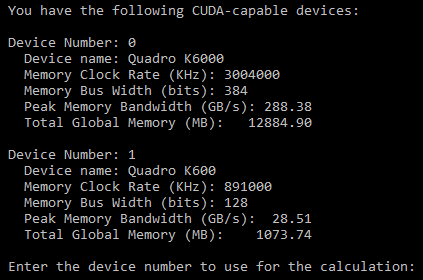
\includegraphics[scale=0.75]{Figures/GPU.png}
\caption{An example of how the GPU selection summary might appear, depending on your system.}
\label{fig:GPU}
\end{center}
\end{figure}

Note: if you are connecting to a remote machine via a Remote Desktop protocol, the program may become confused about which machine it is running on (it may for example present you with a list of graphics cards on the local machine, rather than the remote machine).
In this instance it is recommended that the user connect via SSH instead.
On Windows, an SSH server can be set up using Bitvise SSH.

\subsubsection{GPU memory usage}

The memory requirements of the calculation will be presented to the user prior to the calculation beginning.
If the required memory is greater than that available on the selected device, then the calculation of transmission functions will be done ``on-the-fly'' to minimise memory usage.
The user also has the choice to force on-the-fly calculations.
This option not recommended as it is significantly slower.
However, if the memory requirements have been underestimated the program will crash, and the user is advised to try on-the-fly calculations to see if that helps.
Figure \ref{fig:GPU_memory} depicts a situation where there appears to be enough memory, but on-the-fly calculation has been selected anyway.

\begin{figure}[!h]
\begin{center}
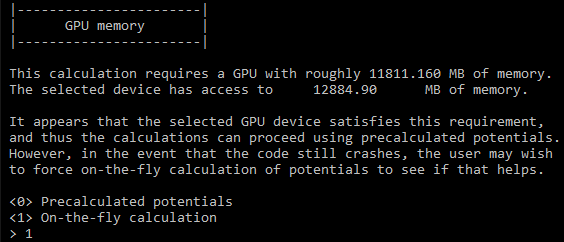
\includegraphics[scale=0.75]{Figures/GPU_memory.png}
\caption{GPU memory requirements}
\label{fig:GPU_memory}
\end{center}
\end{figure}

\subsection{Output filename prefix}

The user may specify a prefix which is used for all data files outputted by the program.
This is helpful to keep datasets organised.

{\bf Recommendation}: $\mu$STEM can be directed to output to a different directory by adding the relative path to the output filename prefix, use this to better organise $\mu$STEM outputs.

\subsection{Specimen input}

The program will next ask the user to enter the name of an .xtl file to define the specimen.
More details about this can be found in Sec. \ref{xtl_input}.

\subsection{Specimen slicing and thickness \label{sec:thickness}}

The user can specify whether or not the unit cell will be divided into slices (along the c-axis of the input structure).
The fractional depths of the \emph{front} faces of each slice can be entered manually or be calculated automatically.
In the latter case the unit cell is divided into slices of uniform thickness.

The distance over which the projection is applied should be kept to less than 2 {\AA} (based on the experience of the authors).
Convergence of the slicing procedure can be checked by simply slicing more finely.
Specimens with no repeat in the $z$-direction (e.g. nano-particles) will require that slicing be used, since in those cases the ``unit cell'' will generally extend far beyond 2 \AA{}.
The experience of the authors suggests that for calculations using the QEP model, slicing can be very important.

If no slicing is used, then the entire unit cell is projected into a single slice.

If an accurate calculation of Higher Order Laue Zone details is important, then slicing finer than the unit cell should be performed.


As an example, for SrTiO$_3$ oriented down the [001] zone axis the unit cell is 3.905 \AA{} to a side, and so slicing the unit cell is recommended.
Fortunately in this case there are two ``natural'' depths at which atoms occur, namely 0.0 and 0.5.
Slicing the unit cell at these depths will yield an accuate multislice solution, assuming other parameters such as unit cell tiling and grid size are sufficient.

\begin{figure}[!h]
	\begin{center}
		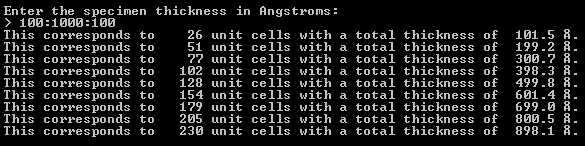
\includegraphics[scale=1.0]{figures/thickness_series.png}
		\caption{User input to $\mu$STEM to perform a thickness series.}
		\label{fig:thickness_series}
	\end{center}
\end{figure}
The specimen thickness is entered in \AA{}ngstr\"om units.
This will be rounded to the nearest thickness that is an integer number of unit cell repeats in the $z$-direction.
Thicknesses can be entered as a single value, a list
($ z_1,z_2,z_3...z_n $)
or a sequence
($ z_{\rm initial}:z_{\rm final}:z_{\rm step}  $).
As an example a thickness series in steps of 100 \AA\, entered as a sequence ($ z_{\rm initial}=100\AA:z_{\rm final}=1000\AA:z_{\rm step}=100\AA  $), is demonstrated in Fig.~\ref{fig:thickness_series}.



\subsection{Potential calculation method}
\label{sec:pot_calc}

\begin{figure}[!h]
\begin{center}
    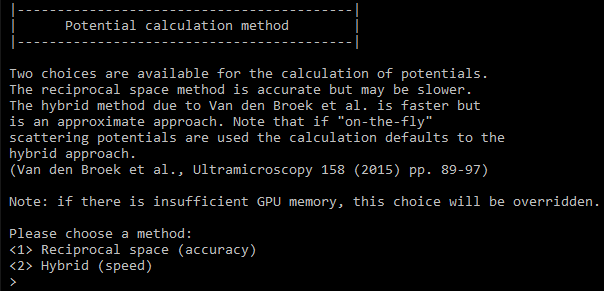
\includegraphics[scale=0.75]{Figures/potential_method.png}
\caption{Choice between potential calculation methods.}
\label{fig:potential_method}
\end{center}
\end{figure}
\begin{figure}
	\centering
	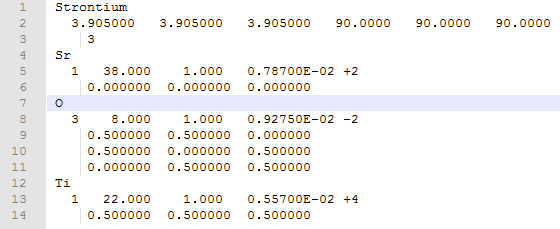
\includegraphics{figures/SrTiO3_ionic.PNG}
	\caption{A \texttt{*.xtl} crystal input file modified to include the ionic state of the atoms within the crystal\label{fig:ionicxtl}}
\end{figure}
Two methods are provided for calculating the potentials: the reciprocal space method and the hybrid method \cite{VDB}.
The reciprocal space method is accurate, while the hybrid method is considerably faster but is not as accurate.
For rapid computations we recommend the hybrid approach, which can be subsequently checked with the reciprocal space method.

Note that if the memory on your graphics card is insufficient for storing pre-calculated potentials for QEP model calculations, then potentials will be calculated ``on-the-fly'' using the hybrid approach.

\subsection{Ionic potentials}
%
By default atomic potentials are calculated within an isolated atom approximation (IAM) using the parametrization of Waasmaier and Kirfel~\cite{WK1}. Ionic bonding can be approximated in $\mu$STEM using by running the program with the command line option \texttt{ionic}. In this case the atomic potentials will be calculated using the parametrisation of Peng~\cite{peng1998electron}, the \texttt{*.xtl} crystal input file will need to be modified to include the ionic state of the atoms within the crystal as shown in Fig.~\ref{fig:ionicxtl}
%


\subsection{Choice of illumination}

The user will next be presented with a choice between plane wave and convergent-beam illumination, which should look like Fig. \ref{fig:illum_choice}.

\begin{figure}[!h]
\begin{center}
    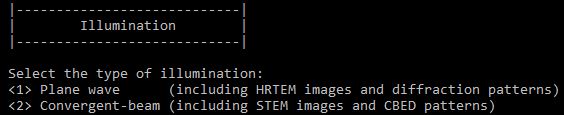
\includegraphics[scale=0.75]{figures/illumination_choice.png}
\caption{Choice of illumination.}
\label{fig:illum_choice}
\end{center}
\end{figure}

Plane wave illumination can be used to calculate images and diffraction patterns within both the QEP and absorptive models.
Convergent-beam illumination can be used to calculate CBED patterns, PACBED patterns and STEM images (including BF/ADF/EDX/EELS) within the QEP and absorptive models.

\subsubsection{Lens aberrations and defocus series}
%
The probe forming aperture is set and Defocus, 3rd and 5th order spherical, twofold and threefold astigmatism and coma aberrations can be included using the lens menu. The form of the lens menu is the same for the probe forming lens in STEM and CBED and the image forming lens in CTEM. A defocus series can be set up in a manner similar to thickness series (see Sec.~\ref{sec:thickness}). Defocus can be entered as a single value, a list
($ \Delta f_1,\Delta f_2,\Delta f_3...\Delta f_n $)
or a sequence
($ \Delta f_{\rm initial}:\Delta f_{\rm final}:\Delta f_{\rm step}  $).
As an example a defocus series in steps of 20 \AA\, entered as a sequence ($ \Delta f_{\rm initial}=-120\AA:\Delta f_{\rm final}=100\AA:\Delta f_{\rm step}=20\AA  $), is demonstrated in Fig.~\ref{fig:lens_parameters}. Note that defocus series have not yet been implemented for the CBED and PACBED routines. These routines will simply take the first defocus in the series.
%
\begin{figure}[!h]
	\begin{center}
		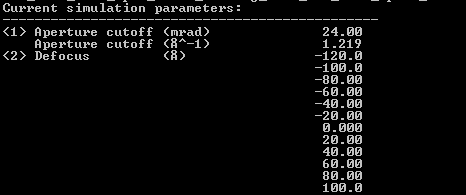
\includegraphics[scale=1.0]{figures/lens_parameters.png}
		\caption{Choice of lens parameters.}
		\label{fig:lens_parameters}
	\end{center}
\end{figure}
%
\begin{figure}[!h]
	\begin{center}
		\includegraphics[width=\textwidth]{figures/aberrations.png}
		\caption{Example output for the phase of the lens contrast transfer function and the intensity of the point spread function. The scale bars were added in ImageJ.}
		\label{fig:aberrations}
	\end{center}
\end{figure}
The menu also offers the option to output the lens constrast transfer function, this is demonstrated for the example of a 24 mrad probe forming aperture with 5000 \AA\ of coma in Fig.~\ref{fig:aberrations}. The phase of the contrast transfer function and the intensity of the real space point-spread function associated with the lens is outputted. In the case of STEM imaging the intensity of the real space point spread function represents the intensity of the STEM probe on the surface of the sample.

There are two things to keep in mind regarding input of aberrations:
\begin{itemize}
	\item The magnitude of all aberrations is in \AA ngstr\"om units for consistency and this can be inconvenient for aberrations above first order such as spherical aberration $C_{30}$ (for which mm is a more convenient unit). Here it is best to use the exponent symbol ``E'' for input, so 1.2 mm of $C_{30}$ is inputted as ``1.2E7'' \AA.
	\item For an uncorrected instrument with significant 3$^{\rm rd}$ order spherical aberration $C_{30}$,  $C_{30}$ should be balanced with defocus $\Delta f $ in the Sherzer condition:
	\begin{align}
	\Delta f = -\mathrm{sgn}(C_{30})\sqrt{4|C_{30}|/3}
	\end{align}
	Where $\mathrm{sgn}(C_{30})$ is the sign of the 3$^{\rm rd}$ order spherical aberration coefficient. As shown in Fig.~\ref{fig:sherzer}, if $C_{30}$ is adjusted, $\Delta f $ should be changed again and $\mu$STEM will automatically suggest the appropriate Sherzer condition.
	\begin{figure}
		\includegraphics{figures/sherzer.png}
		\caption{For a given 3$^{\rm rd}$ order spherical aberration $C_{30}$ $\mu$STEM will suggest the appropriate Sherzer defocus condition\label{fig:sherzer}}
	\end{figure}
\end{itemize}

%
\begin{figure}[!h]
	\begin{center}
		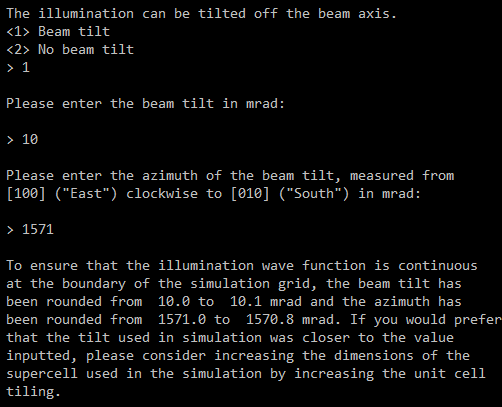
\includegraphics[scale=1.3]{figures/tilt_beam.png}
		\caption{Tilting the beam (illumination)}
		\label{fig:tilt_beam}
	\end{center}
\end{figure}
%
\begin{figure}[!h]
	\begin{center}
		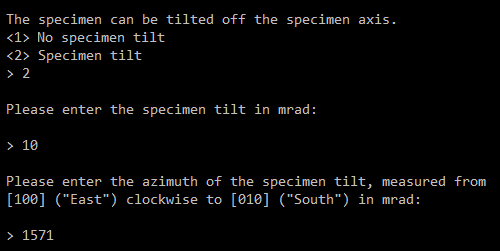
\includegraphics[scale=1.3]{figures/tilt_specimen.png}
		\caption{Tilting the specimen.}
		\label{fig:tilt_specimen}
	\end{center}
\end{figure}

\subsubsection{Tilting the beam (illumination) and/or specimen}

The beam (illumination) can be tilted away from the optical axis and/or the specimen can be tilted (new feature in v4.6). In Fig. \ref{fig:tilt_beam} we show an example where the beam is tilted and in Fig. \ref{fig:tilt_specimen} the specimen is tilted. Tilts of up to a few degrees can be handled in this way.



\subsection{Thermal scattering model}

The user will next have a choice between two scattering models.
Briefly, the absorptive model permits a rapid calculation but only considers how thermal scattering attenuates the elastic wave function.
Thermal scattering cross sections are calculated in a single inelastic scattering approximation, less accurate for thicker specimens.
Channelling of the thermally scattered electrons is also ignored.

The Quantum Excitation of Phonons (QEP) model includes all thermal scattering effects but will take longer to calculate.
More details are given below.

\subsubsection{Absorptive model}
\label{sec:absorptive}

The absorptive model is a method of including the effects of thermal scattering on the \emph{elastic} wave function, by attenuating the wave function with the ``absorption'' due to thermal scattering.
The contributions made by those electrons which have been thermally scattered are \emph{not} included in many of the results.
Exceptions to this are STEM images for diffraction plane detectors, which include thermal scattering in the single inelastic scattering approximation.
For thicker specimens, multiple thermal scattering becomes significant and the QEP model should be used instead.

The user may also choose to not include absorption at all, in which case no thermal scattering is considered.
The atomic potentials will still however be ``smeared out'' according to the temperature factors specified in the xtl file.
This option is useful for checking if the grid size is sufficient.
The intensity displayed in the status line during calculation will drop below 1.0 if electrons are being ``lost'' due to inadequate numerical parameters, namely the grid size.


\subsubsection{QEP model}
\label{sec:qep}


The Quantum Excitation of Phonons (QEP) model \cite{Forbes2010} is a rigorous approach to handling what is also known as thermal diffuse scattering (TDS).
The advantages of this model are its quantum mechanical underpinnings and the fact that we can keep track of electrons which have been elastically scattered and thermally scattered separately.
This means that the contribution to EELS and EDX due to both elastically and thermally scattered electrons can be tracked separately.

If one is not interested in the contribution from thermally scattered electrons to EELS and EDX cross sections, then an absorptive model calculation would suffice.
In fact, the elastic contribution will be very similar to that calculated in the QEP, and will be significantly faster to calculate within the absorptive model.
Nevertheless, the thermally scattered component is often crucial in understanding the physics \cite{Forbes2012}.

Calculations of the total scattered intensity in the QEP model are numerically equivalent to what would be obtained in a frozen phonon (FPh) model calculation \cite{LXS}; for the FPh mode, the separation into elastic and thermal components is not obvious.

\paragraph{Practical considerations}

Using the QEP model typically requires the unit cell to be tiled out by at least 4\by4.
Additionally, the atomic potentials are not thermally smeared out as in the absorptive model but rather are quite sharp, which corresponds to requiring a large grid size that permits high-angle scattering.
The user should ensure that their choice of grid size allows scattering out to at least 150 mrad, or at the very least confirm convergence of their results by using progressively larger grid sizes.
The user can also monitor the intensity at each probe position to ensure that it does not drop significantly below 1.0.

The algorithm employed by the QEP model relies on displacing the atoms in the specimen into a number of random configurations based on the thermal motion of the atoms.
The accuracy of the QEP calculation increases as more configurations are chosen; as a loose rule of thumb the authors would recommend at least 40 configurations.
More than 100 passes may be required for the elastic contribution to reach convergence.
Precalculating many transmission functions may require a large amount of memory.

To ameliorate this, the program can randomly translate the transmission functions by an integer number of unit cells in each direction.
Whilst technically this is not a different configuration, it may effectively be different as seen by the incident electron wave function.
Using this approach increases the number of configurations by a factor equal to the number of unit cells that have been tiled out.
The translation of transmission functions is computationally fastest when there are an integer number of pixels along each direction of the unit cell.
For example, with a 4\by4 tiling and a 512\by512 grid size, there are 128\by128 pixels per unit cell.
If this is not the case then the code must revert to using the Fourier Shift theorem and this will cost, in computational terms, an extra FFT per slice.

It is also possible to generate transmission functions ``on-the-fly'', which means that transmission functions are not precalculated but rather are calculated just before they are needed, and then are discarded.
While slower than the precalculation approach it does significantly reduce memory requirements and allows the simulation of aperiodic systems containing of the order of 10$^{6}$ atoms.
This option is only used if the GPU does not have sufficient memory to precalculate and store an adequate number of transmission functions.

The user may also specify the ``starting position of the random number sequence''.
Normally this input is not important, and any integer can be entered.
If the same number is entered for the same inputted parameters, then the results of the calculation should be numerically identical.
This is useful for exactly reproducing results, e.g. for checking purposes.



\subsection{Tiling and grid size}

\subsubsection{Unit cell tiling}
\label{sec:tiling}

The user may specify how the unit cell is tiled to form a supercell.
This is necessary in two cases: where the QEP model is being used, or when the illumination is a convergent beam (e.g. a STEM probe).
In the former case, we recommend that the tiling is at least a factor of 4 in each direction, although if the unit cell (as specified in the xtl file) is a complicated structure such as a nano-particle or an interface, it may already be large enough so that tiling is not needed.
In the case of convergent-beam illumination, it is important that the supercell is large enough so that the scattered probe wave function does not ``wrap around'' the supercell and interfere with itself.
A supercell with side lengths of 30 \AA{} should be sufficient to contain a atom-sized probe (e.g. probe-forming convergence semi-angle of 15 mrad for 300 keV electrons, which gives a probe about 1 \AA{} across).

If the absorptive model is being used and the illumination is a plane wave, then no tiling is necessary.

For further details on supercell tiling please review Ref. \cite{FAOR1}. 

\subsubsection{Size of the grid}

The user must also specify the number of pixels on the grid on which calculations will proceed.
The size of this grid (in conjunction with the unit cell tiling) determines the resolution of the calculation, or equivalently, it determines the plane wave basis with which the calculation will proceed.
An important consideration is that this plane wave basis should extend out far enough to cover the possible range of outgoing wave vectors.
If it is insufficient, then electrons scattered to high angles will not contribute appropriately to the calculation.
This will affect primarily calculations of annular dark field STEM images in the QEP model.

Once the tiling and grid size have been specified, the program will output a number of derived quantities, which include the maximum scattering vectors/angles included in the calculation.
It is important to review these numbers to ensure that they are sufficient for the desired calculation.

There are further considerations when choosing the size of the grid:
%
\begin{itemize}
    \item Pixel numbers (in each direction) that are products of powers of small primes can result in significantly faster calculations, since the majority of the time is spent performing Fast Fourier Transforms.
        The optimal choice would be a power of 2, e.g. 64, 128, 256, 512, 1024 etc.

    \item Calculations within the QEP model may be sped up significantly if there is an \emph{integer} number of pixels per unit cell, since in that case we can effectively compute new ``frozen lattice'' configurations by simply translating an entire transmission function by a random physical lattice vector, which would correspond to an integer number of pixels.
        Otherwise, one would need to compute significantly more transmission functions (taking up more memory and time) or translate the transmission functions using a phase ramp in Fourier space (i.e. applying the Fourier Shift Theorem) which is less efficient.
\end{itemize}

\paragraph{Comments:}

One can check whether the size of the grid is sufficient by monitoring the intensity which is output as the calculation runs.
If the intensity drops significantly below 1.0, then the grid size could be increased.
To check this for calculations using the absorptive model, one should initially choose the option ``Do not include absorption'' and check that the intensity is sufficiently conserved.
Subsequently the calculation should be run with absorption included.


\subsection{Saving and loading transmission functions}

New in version 4.4 is the ability to save and load precalculated transmission functions.
The associated files may require a large amount of disk space, depending on the calculation.
These can be loaded for subsequent calculations provided the following parameters are identical:
%
\begin{itemize}
    \item The xtl file
    \item The slicing of the unit cell
    \item The choice of thermal scattering model (QEP vs. absorptive)
    \item The tiling of the unit cell
    \item The number of pixels
    \item (For absorptive model: whether absorption is included)
    \item (For QEP model: the number of distinct transmission functions)
    \item (For QEP model: phase ramp shift choice)
\end{itemize}
%
Saving the transmission functions is depicted in Fig. \ref{fig:save_grates}.
The transmission functions are stored in a file prefixed according to the user's specification at the beginning of the program.
In a subsequent calculation, the user can choose to load these transmission functions by specifying the filename.


\begin{figure}[!h]
\begin{center}
    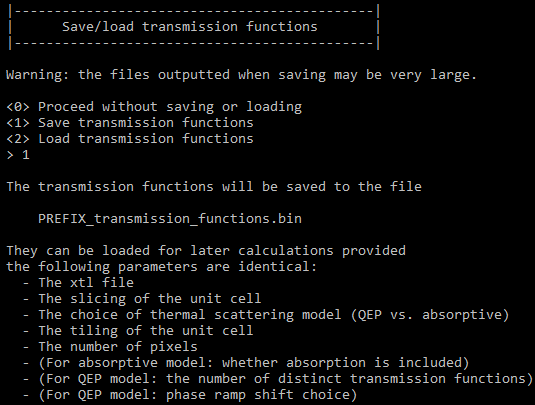
\includegraphics[scale=0.75]{figures/save_grates.png}
\caption{Saving transmission functions to file}
\label{fig:save_grates}
\end{center}
\end{figure}

\subsection{Remaining choices}

The choices remaining to the user are specific to each type of calculation, and will be covered in the case studies in the following section.




\section{Case studies}

In this section we present a few case studies with specific details about what typical choices of parameters might be. For more worked examples of $\mu$STEM calculations and a simple worksheet see the \href{https://github.com/HamishGBrown/MuSTEM/tree/master/Tutorial}{Tutorials} folder on the GitHub.

\subsection{Plane wave illumination with the absorptive model}
\label{sec:abs_hrtem}

For this example we will use the case study of SrTiO$_3$ (STO) with 300 keV plane wave illumination oriented down the $\langle 001 \rangle$ zone axis.
The .xtl file is provided with the program under the name \verb|SrTiO3_001_300keV.xtl|.
After entering this filename at the prompt, details of the specimen will be written to the screen.
The user is advised to check the values here to ensure that they are sensible.

This specimen has a repeat distance of 3.905 \AA{} in the $z$-direction, which could potentially introduce a significant error in the multislice calculation.
We will thus slice the unit cell.
Since there are atoms sitting at only two depths, 0.0 and 0.5, we will choose these manually, as depicted in Fig. \ref{fig:pw_abs_slicing}.

For this example the thickness is assumed to be 200 \AA{}.
After this is entered, the program outputs how many unit cells will be used and the corresponding thickness.
In this case, rounding to the nearest thickness corresponding to a whole number of unit cells gives 199.2 \AA{}.
    
\begin{figure}[!h]
\begin{center}
    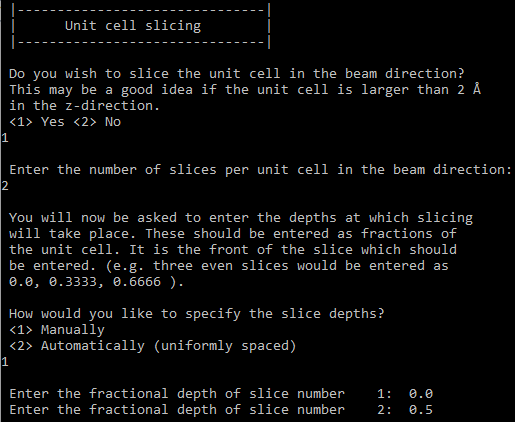
\includegraphics[scale=0.75]{figures/pw_abs_slicing.png}
\caption{Slicing choices}
\label{fig:pw_abs_slicing}
\end{center}
\end{figure}

The next prompt is a choice between two methods of calculating potentials: the reciprocal space method and the hybrid method.
For this example we choose the reciprocal space method since it is the most accurate and will not take too long for this example.
For more details on this topic see Sec. \ref{sec:pot_calc}.

We then choose the options for ``Plane wave illumination'' and ``Absorptive model''.
At this point you will be prompted to enter details of unit cell tiling and grid size.
%
\begin{figure}[!h]
\begin{center}
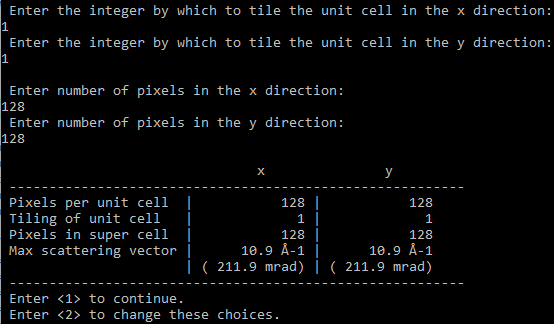
\includegraphics[scale=0.75]{figures/pw_abs_numerical.png}
\caption{A summary of a smeared HRTEM calculation supercell setup.}
\label{fig:pw_abs_numerical}
\end{center}
\end{figure}
%
This calculation assumes a perfectly periodic crystal and illumination and hence does not require a supercell.
A typical choice of numerical sampling parameters is depicted in Fig.~\ref{fig:pw_abs_numerical}.
A grid size of $128\times128$ has been chosen which, for the $1\times1$ unit cell tiling means that the \emph{elastic} wave function will be computed out to a scattering angle of 211~mrad. 
Experience suggests that for plane wave illumination this is more than sufficient, the reasons for this being twofold:
%
\begin{enumerate}
    \item{If we are calculating an HRTEM image we would typically include an aperture on the image-forming lens, which will most likely correspond to scattering angles far less than 211~mrad.}
    \item{For specimen thicknesses typically used for atomic resolution HRTEM, the smeared elastic scattering potential will generally not scatter a significant fraction of the incident flux to angles greater than 100~mrad.}
\end{enumerate}
%
The user is encouraged to check that the grid size is sufficient by running a calculation in the absorptive model but with absorption switched off, for more details see Sec. \ref{sec:absorptive}.



%\begin{figure}[!h]
%\begin{center}
%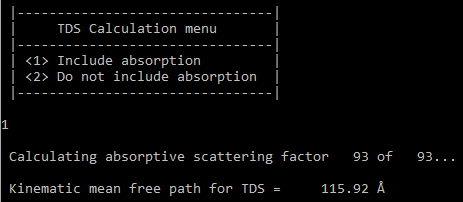
\includegraphics[scale=0.75]{pw_abs_TDS.png}
%\caption{TDS calculation}
%\label{fig:pw_abs_TDS}
%\end{center}
%\end{figure}
%
%We now choose to include the effect of TDS (Fig. \ref{fig:pw_abs_TDS}). 
%Electing not to include absorption due to TDS will still construct the correct elastic scattering potential (appropriately smeared to account for the time average) however, the elastic wave function will not contain the effect that inelastic phonon scattering has upon it.
%The reason to perform this calculation is to provide a facility to check whether the chosen grid size is sufficient (see comments earlier).
%The program will also tell us the kinematic mean free path for thermal scattering.
%If the thickness is much greater than this mean free path, then multiple thermal scattering may become significant, in which case the QEP model should be used instead.

\begin{figure}[!h]
\begin{center}
    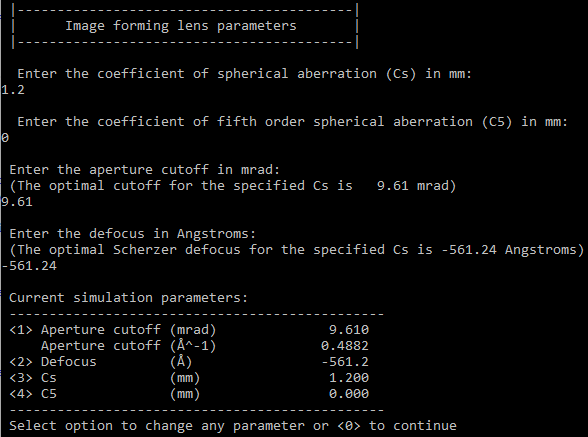
\includegraphics[scale=0.75]{figures/pw_abs_lens.png}
\caption{A summary of the image forming lens parameters.}
\label{fig:pw_abs_lens}
\end{center}
\end{figure}

The user will now be presented with a series of questions pertaining to the imaging lens of the microscope (see Fig. \ref{fig:pw_abs_lens}). 
In this example we have used a $C_\text{s}$ of 1.2 mm, and have accepted the recommended aperture cutoff and defocus to optimise for phase constrast in the image.
The sign convention for defocus is such that a positive value indicates more `focusing' power (overfocus). 
In other words the wave is brought to a focus before the detector plane.  

The program will now compute the image and diffraction pattern (see Fig. \ref{fig:pw_abs_calc}) and output these 2D images as files named in the following format:
%
\begin{myenv}
    \verb|<Prefix>_Image_<NX>x<NY>.bin| \\
    \verb|<Prefix>_DiffractionPattern_<NX>x<NY>.bin|
\end{myenv}
%
where \verb|NX| and \verb|NY| are the dimensions of the 2D image.

\begin{figure}[!h]
\begin{center}
    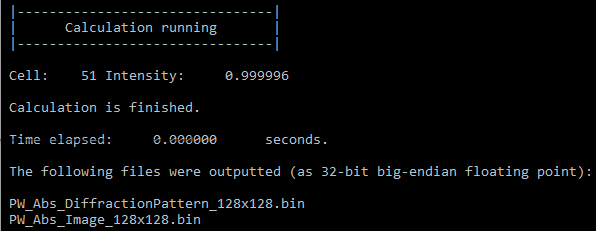
\includegraphics[scale=0.75]{figures/pw_abs_calc.png}
\caption{Calculation output.}
\label{fig:pw_abs_calc}
\end{center}
\end{figure}

To load these files in ImageJ, go to File $\rightarrow$ Import $\rightarrow$ Raw, locate the file, and enter the details shown in Fig. \ref{fig:ImageJ_ImportRaw} (note that the single precision version has been used for this example and hence the ``Image type'' is ``32-bit Real'').

\begin{figure}[!h]
\begin{center}
    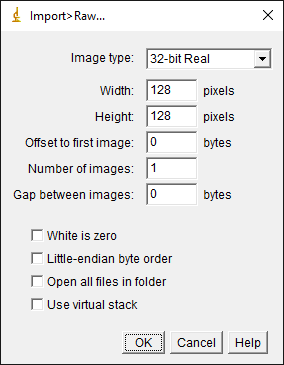
\includegraphics[scale=0.75]{figures/ImageJ_ImportRaw.png}
    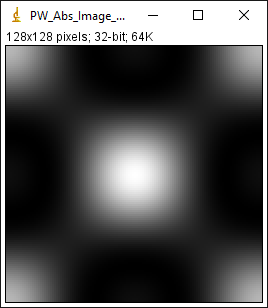
\includegraphics[scale=0.75]{figures/pw_abs_image.png}
\caption{Loading a binary file in ImageJ. The HRTEM image is displayed.}
\label{fig:ImageJ_ImportRaw}
\end{center}
\end{figure}

A more convenient way to load the files is using the \href{http://imagejdocu.tudor.lu/doku.php?id=plugin:utilities:droplet:start}{Droplet: Drag and Drop file processor} plugin written by Jerome Mutterer and Wayne Rasband for ImageJ. Follow the link and download instructions therein for the Droplet Plugin then add the contents of the \href{https://github.com/HamishGBrown/MuSTEM/tree/master/Auxiliary_tools/Droplet Actions}{\emph{Droplet Actions}} folder from the muSTEM github to the folder of the same name in the \emph{plugins} directory of your ImageJ directory. A screenshot of the droplet app is shown in Fig.~\ref{fig:ImageJ_Droplet}.
\begin{figure}[h!]
	\begin{center}
		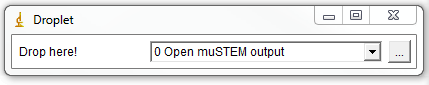
\includegraphics[scale=0.75]{figures/ImageJ_droplet.png}
		\caption{The ImageJ droplet with scripts to open $\mu$STEM output: a much more convenient way of viewing data\label{fig:ImageJ_Droplet}}
	\end{center}
\end{figure}

If you use either Matlab\textsuperscript{TM} or Python programming languages for data analysis then functions to open $\mu$STEM output in these languages are also available in the \href{https://github.com/HamishGBrown/MuSTEM/tree/master/Auxiliary_tools}{\emph{Auxiliary$\_$tools}} folder

The diffraction pattern does not usually look very interesting when first displayed.
It is often necessary to adjust contrast or apply a log transformation.
We refer the user to the ImageJ documentation and to the literature for this.

\subsection{Plane wave illumination with the QEP model}
\label{qep_hrtem}

A plane wave QEP calculation proceeds largely as per Sec. \ref{sec:abs_hrtem}. 
The differences between the two calculation approaches will be discussed presently.

\begin{figure}[!h]
\begin{center}
    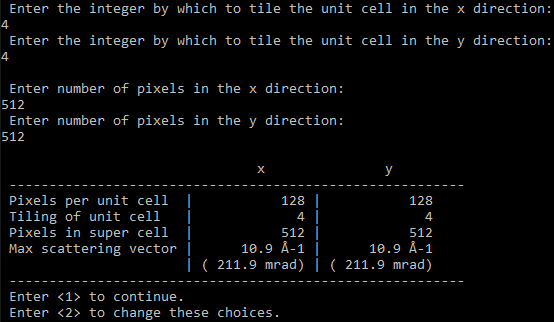
\includegraphics[scale=0.75]{figures/pw_qep_numerical.png}
\caption{Numerical parameters for plane wave illumination and QEP model}
\label{fig:pw_qep_numerical}
\end{center}
\end{figure}

As discussed in Sec. \ref{sec:tiling}, the unit cell must be tiled out for calculations in the QEP model, and consequently the grid size must be increased to ensure that high angle scattering is correctly accounted for.
In this example we will use a 4\by4 tiling and 512\by512 pixels.
This is depicted in Fig. \ref{fig:pw_qep_numerical}, and we can see that scattering is included out to 212 mrad, which should be sufficient.
These numerical parameters have the further advantage that there are an integer number of pixels per unit cell (128 in each direction).
As discussed in Sec. \ref{sec:qep} this speeds up the calculation and saves memory by allowing the precalculated transmission functions to be quick shifted by random physical lattice vectors to effectively gain new transmission functions.

\begin{figure}[!h]
\begin{center}
    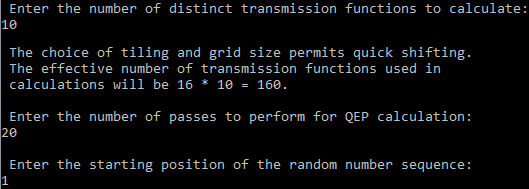
\includegraphics[scale=0.75]{figures/pw_qep_qep_questions.png}
\caption{QEP parameters}
\label{fig:pw_qep_qep_questions}
\end{center}
\end{figure}

The user will now be asked some specific questions relating to the QEP model.
In Fig. \ref{fig:pw_qep_qep_questions} we show the numbers used in this example; 10 distinct transmission functions have been calculated, but since quick shifting is possible in this case, there will effectively be 160 configurations.
This should be more than sufficient.
We have chosen to use 20 passes, which should usually be sufficient for calculating the total scattered intensity.
However, it may be insufficient for calculation of elastic intensities (and thermal intensities, which are calculated by subtracting the elastic from the total).
The absorptive model can be used for rapid calculation of elastic intensities.
The number chosen as the starting position of the random number sequence is only important for reproducing a previous result, and can be any integer.

At this point the user will be asked to specify the parameters of the image forming lens, for more details Fig. \ref{fig:pw_abs_lens} and the surrounding discussion.

The program will now calculate the transmission functions and then proceed with the multislice solution.
At completion the code will output the exit surface elastic intensity and phase, the inelastic intensity and the total intensity. It will also output the equivalent far-field diffraction and image plane quantities. 

The following files are outputted:
%
\begin{myenv}
    \verb|<Prefix>_DiffPlaneTotal_<NX>x<NY>.bin| \\
    \verb|<Prefix>_DiffPlaneElastic_<NX>x<NY>.bin| \\
    \verb|<Prefix>_DiffPlaneTDS_<NX>x<NY>.bin| \\
    \verb|<Prefix>_ExitSurface_IntensityElastic_<NX>x<NY>.bin| \\
    \verb|<Prefix>_ExitSurface_PhaseElastic_<NX>x<NY>.bin| \\
    \verb|<Prefix>_ExitSurface_IntensityTotal_<NX>x<NY>.bin| \\
    \verb|<Prefix>_ExitSurface_IntensityTDS_<NX>x<NY>.bin| \\
    \verb|<Prefix>_Image_Elastic_<NX>x<NY>.bin| \\
    \verb|<Prefix>_Image_TDS_<NX>x<NY>.bin| \\
    \verb|<Prefix>_Image_Total_<NX>x<NY>.bin|
\end{myenv}



\subsection{Convergent beam illumination with the absorptive model}
\label{abs_stem}

A calculation using a convergent beam and the absorptive model proceeds similarly to the plane wave illumination procedure outlined in Sec. \ref{sec:abs_hrtem} with a few exceptions detailed here.

\begin{figure}[!h]
\begin{center}
    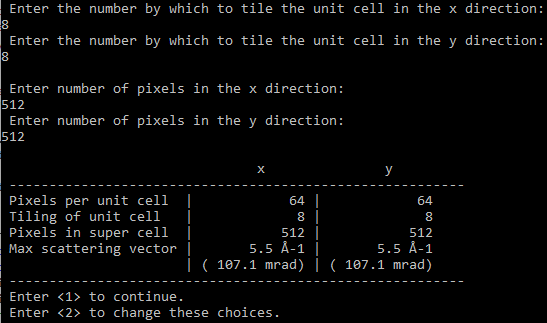
\includegraphics[scale=0.75]{figures/cb_abs_numerical.png}
\caption{Typical numerical parameters for a convergent beam calculation using the absorptive model.}
\label{fig:cb_abs_numerical}
\end{center}
\end{figure}

As the convergent probe does not share the same periodicity as the crystal we require the use of a supercell.
The size of the supercell must be such that there is no ``aliasing'' of the probe, which occurs when the probe wave function scatters and subsequently extends to the edges of the supercell.
Numerical tests for aliasing are not easily defined and we are forced to rely on intuition.
As a general rule of thumb the more scattering that occurs the larger the supercell needs to be.
Another rule of thumb is that the finer the probe is the larger the supercell needs to be.
Without being prescriptive, keeping the supercell side lengths larger than 30{\AA} is usually sufficient, the caveat being that larger is usually better. 
If in doubt, the user is encouraged to double the tiling of the unit cell and simultaneously double the grid size, which will increase the size of the supercell while keeping the resolution of the simulation constant.

In the present case study, we have tiled the STO unit cell 8\by8 so that the supercell measures 31 \AA{} \by{} 31 \AA{}.
We use a grid size of 512\by512, which should be sufficient for the absorptive model.
This should be checked in practice by doubling the grid size to 1024\by1024 and checking the results.
These parameters are depicted in Fig. \ref{fig:cb_abs_numerical}.

\begin{figure}[!h]
\begin{center}
    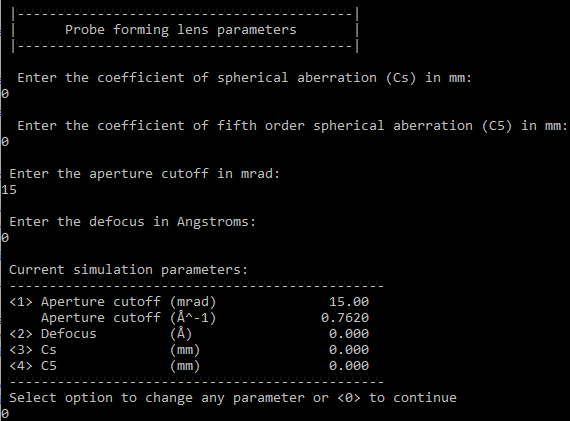
\includegraphics[scale=0.75]{figures/cb_abs_lens.png}
\caption{Parameters for the probe-forming lens.}
\label{fig:cb_abs_lens}
\end{center}
\end{figure}

The probe-forming lens is set up in much the same way as for an imaging lens, as described in Sec. \ref{sec:abs_hrtem} and depicted in Fig. \ref{fig:cb_abs_lens}.
In this case we have assumed an aberration-corrected probe with a convergence semi-angle of 15 mrad.



\begin{figure}[!h]
\begin{center}
    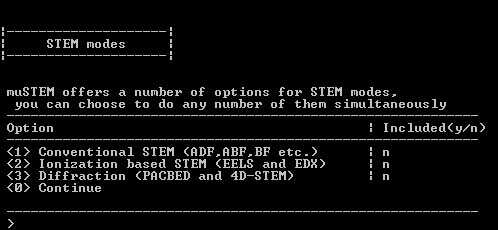
\includegraphics[scale=0.75]{figures/cb_abs_types.png}
\caption{Choosing the type of convergent-beam calculation to perform.}
\label{fig:cb_abs_types}
\end{center}
\end{figure}

The user is now presented with a list of possible calculations as depicted in Fig. \ref{fig:cb_abs_types}.
These calculation types are explained in the following sections.



\subsubsection{CBED patterns}

The user will be asked to enter the fractional co-ordinate, with respect to the unit cell, to place the probe.
In this case, we position the probe over the strontium-containing column and thus specify ``\verb|0.0 0.0|''.
The CBED pattern will be outputted with the filename in the form
%
\begin{myenv}
    \verb|<Prefix>_DiffractionPattern_<NX>x<NY>.bin| \; .
\end{myenv}
%



\subsubsection{PACBED patterns} 

The calculation will proceed using the probe positions determined from the information transfer limit of the microscope and the unit cell under consideration.
A choice is given as to whether to output the different diffraction patterns contributing toward the PACBED.
If pertinent these will be outputted with the filename in the form
%
\begin{myenv}
	\verb|<Prefix>_pp_<n_x>_<n_y>_Diffraction_pattern_<NX>x<NY>.bin| \; .
\end{myenv}
where the integers $\verb|<n_x>|$ and $\verb|<n_y>|$ label the scan positions of the probe across the unit cell.
This option allows one to construct a ``4D STEM'' data-set, ie one that could be achieved in experiment with a fast-readout pixelated detector.
The PACBED pattern will be outputted with the filename in the form
%
\begin{myenv}
    \verb|<Prefix>_PACBED_Pattern_<NX>x<NY>.bin| \; .
\end{myenv}



\subsubsection{STEM images}

The STEM probe intensity can optionally be outputted as a function of thickness at each probe position.
This is depicted in Fig. \ref{fig:probe_intensity}.
The resulting dataset may be very large.



\begin{figure}[!h]
\begin{center}
    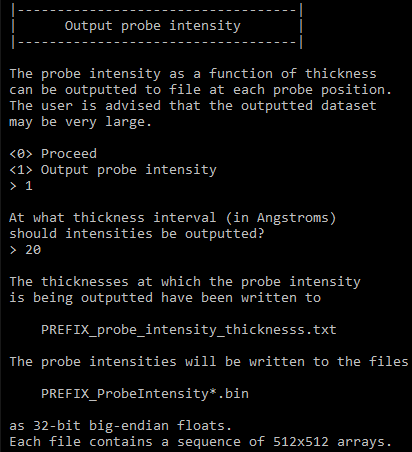
\includegraphics[scale=0.75]{figures/probe_intensity.png}
\caption{Outputting the STEM probe intensity.}
\label{fig:probe_intensity}
\end{center}
\end{figure}

When calculating \emph{any} type of STEM image, the user can choose the inner and outer angles for a number of detectors in the diffraction plane, so that for example a STEM HAADF image can be simultaneously calculated.
These angles can be chosen to simulate a broad range of imaging modes, including bright-field (BF), annular bright field (ABF) and annular dark field (ADF) simultaneously.
Segmented detectors are also a possibility and can be accessed by inputting the number of detector annular and angular segments seperated by a comma.
Input for a 4 annulus \by 4 segment detector system is shown by way of example in Fig.~\ref{fig:detectors}.
For all examples in the following sections, we specify a HAADF detector with inner and outer angles of 60 and 180 mrad respectively.

\begin{figure}[!h]
	\begin{center}
		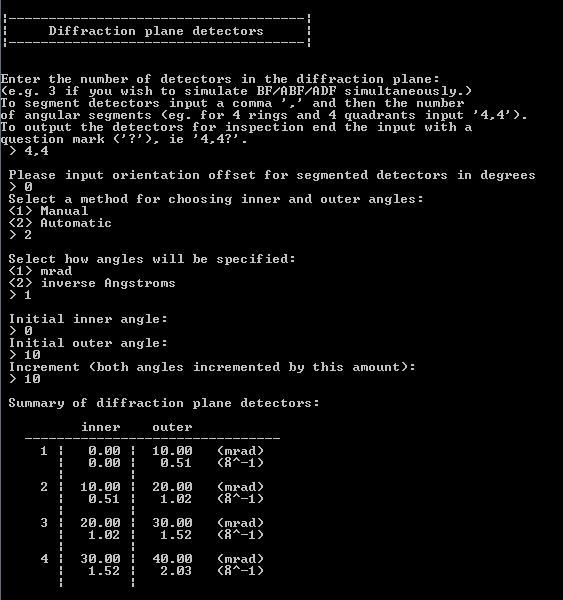
\includegraphics[scale=0.75]{figures/Detectors.PNG}
		\caption{Choosing STEM detectors in $\mu$STEM.}
		\label{fig:detectors}
	\end{center}
\end{figure}


\subsubsection{STEM EELS images}

\begin{figure}[!h]
\begin{center}
    \includegraphics[scale=0.75]{figures/cb_abs_EELS.png}
\caption{Parameters for an EELS calculation}
\label{fig:cb_abs_EELS}
\end{center}
\end{figure}

In this example we have chosen an EELS detector collecting electrons out to 50 mrad.
A correction is applied to account for the finite detector size \cite{Zhu2013}.
We choose to calculate the STEM EELS image that would result from only detecting electrons which have inelastically scattered after ionizing oxygen atoms within the 1s orbital.
We choose an energy window which extends 30 eV above threshold as an example.
See Fig. \ref{fig:cb_abs_EELS}.

Next the user will be prompted for details about scan vectors and probe position sampling.
Typically the defaults should be accepted.
In the present example, that means that there will be 12\by12 probe positions.

The calculated STEM images will also be tiled and interpolated according to the user's specifications.
In the present example we have specified that the image should be interpolated up to a maximum of 100\by100 pixels (the actual output dimensions will depend in general on the aspect ratio of the region over which the probe is scanned), and we have used a 2\by2 tiling.

The template for the outputted filenames is:
%
\begin{myenv}
    \verb|<Prefix>_DiffPlaneTotal_Defocus<DF>_<NX>x<NY>.bin| \\
    \verb|<Prefix>_DiffPlaneElastic_Defocus<DF>_<NX>x<NY>.bin| \\
    \verb|<Prefix>_DiffPlaneTDS_Defocus<DF>_<NX>x<NY>.bin| \\
    \verb|<Prefix>_EELS_Defocus<DF>_<NX>x<NY>.bin| \\
    \verb|<Prefix>_EELS_CorrectionMap_Defocus<DF>_<NX>x<NY>.bin| \\
    \verb|<Prefix>_EELS_Corrected_Defocus<DF>_<NX>x<NY>.bin| \\
\end{myenv}
%
%Deprecated in Version 5.1
%Each of these filenames will run over all specified probe defoci and will additionally have an interpolated version which includes the suffix \verb|_Interpolated|.

\subsubsection{STEM EDX images}

The STEM EDX inputs are slightly different than EELS inputs.
%The user can only choose a shell rather than an orbital.
The concept of an energy window is meaningless here, since the EDX signal is proportional to the probability of an electron being ejected with \emph{any} kinetic energy, hence the energy window effectively extends all the way to the incident energy minus the binding energy.
The EDX image is calculated assuming that the signal comes from electrons that are inelastically scattered through all angles after ionization.
Figure \ref{fig:cb_abs_EDX} depicts the parameters we have chosen for this example.

\begin{figure}[!h]
\begin{center}
    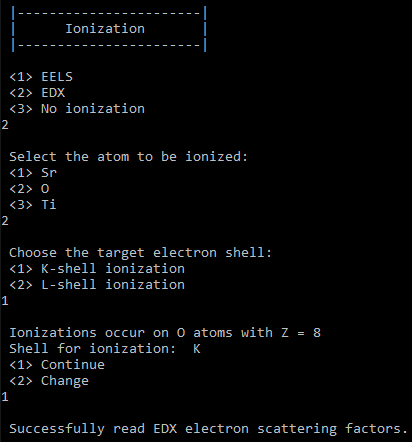
\includegraphics[scale=0.75]{figures/cb_abs_EDX.png}
\caption{Parameters for an EDX calculation}
\label{fig:cb_abs_EDX}
\end{center}
\end{figure}





\subsection{Convergent beam illumination with the QEP model}

A QEP STEM calculation proceeds largely as per Sec. \ref{abs_stem}.
There are QEP specific questions which are discussed in Sec. \ref{qep_hrtem}.
The choice of numerical parameters here is affected by both the requirements of the QEP model and the requirements of a convergent-beam probe.
That is, the unit cell should be tiled out sufficiently so that the probe is ``contained'' within the supercell (see Sec. \ref{abs_stem}) and the grid size should be sufficiently large so that scattering to high angles is included (see Sec. \ref{qep_hrtem}).

Further differences here are that many diffraction plane detectors may be specified and all quantities are outputted as \verb|Total|, \verb|Elastic| and \verb|TDS|, the latter being the contributions from elastic and thermal scattering respectively.

\bibliographystyle{plain}
\bibliography{muSTEM_manual}

\end{document}
